\chapter{Filter}
Filter sind spezielle Systeme, die in diesem Abschnitt
grundsätzlich als LTI-Systeme angenommen werden\footnote{Es gibt
auch nicht-lineare Filter. Ein sehr einfaches Beispiel stellt das
Median-Filter dar.}. Die Aufgabe von Filtern ist bestimmte Anteile
aus dem Signal zu entfernen oder abzuschwächen. Dies kann durch
eine Abschwächung der ungewünschten Signalanteile oder eine
Verstärkung der gewünschten Signalanteile erfolgen.

Alle nicht-trivialen LTI-Systeme erzeugen eine Filterwirkung,
trotzdem werden nicht alle LTI-Systeme als Filter bezeichnet, da
das Ziel beim Entwurf nicht die Filterwirkung sondern irgendeine
andere Eigenschaft ist. Zum Beipiel einen gleitenden Mittelwert zu
berechnen. Eine solches System ist automatisch auch ein Filter,
wird aber trotzdem nicht unbedingt als solches bezeichnet. In
vielen Fällen ist die Filterwirkung sogar ein ungewünschter
Nebeneffekt.

Ziel dieses Abschnittes ist es, die Grundtypen von Filtern kennen
zu lernen. Des weiteren werden wir die beiden Realisierungsformen
als nicht-rekursive und rekursive Implementierung kennen lernen.
Abschließend werden in einer sehr kompakten Form einige bekannte
Entwurfsverfahren für die beiden Realisierungsformen vorgestellt.

\section{Filtertypen}
Bei der Typisierung von Filtern schauen wir uns zunächst die
sogenannten Sperrfilter an. Ihr Entwurfsziel ist, möglichst einen
bestimmten Frequenzbereich vollständig aus dem Spektrum zu
entfernen. Dabei wird zwischen vier Grundtypen unterschieden:
\begin{itemize}
    \item {\bf Tiefpass:} Ziel des Tiefpasses ist es alle hohen
    Frequenzen, ab einer zu definierenden Grenzfrequenz $f_g$ aus dem
    Spektrum zu entfernen. In der technischen Umsetzung ist es
    aber nicht möglich, einen abrupten Übergang zwischen
    dem sog. Durchlassbereich (tiefe Frequenzen beim Tiefpass) und
    dem Sperrbereich zu realisieren. Eine praktische Realisierung
    hat deshalb immer bestimmte Grenz- und Übergangsbereiche.
    \begin{figure}[H]
    \begin{center}
    \includegraphics{psFilt/DesignTP}
    \caption{\label{pic:DesignTP}Optimaler Entwurf eines Tiefpasses ($f_s$ = 8 kHz und
    Grenzfrequenz = $f_g$ = 1 kHz) und Realisierung durch Butterworth-Filter 6. Ordnung
    (siehe Abschnitt \ref{sec:Butterworth})}
    \end{center}
    \end{figure}
    \item {\bf Hochpass:} Das inverse Designziel zum Tiefpass
    liegt dem Hochpassentwurf zu Grunde. Es sollen möglichst alle
    tiefen Frequenzen aus dem Spektrum entfernt werden. Auch hier
    gelten die beim Tiefpass erwähnten Einschränkungen.
    \begin{figure}[H]
    \begin{center}
    \includegraphics{psFilt/DesignHP}
    \caption{\label{pic:DesignHP}Optimaler Entwurf eines Hochpasses ($f_s$ = 8 kHz und
    Grenzfrequenz = $f_g$ = 1 kHz) und Realisierung durch Butterworth-Filter 6. Ordnung
    (siehe Abschnitt \ref{sec:Butterworth})}
    \end{center}
    \end{figure}
    \item {\bf Bandpass:} Im Gegensatz zu den vorher erwähnten
    Typen, hat das Bandpassfilter zwei Grenzfrequenzen $f_1$ und
    $f_2$, da das Designziel ist, nur die Frequenzen zwischen
    $f_1$ und $f_2$ durchzulassen und ale Frequenzen unterhalb von
    $f_1$ bzw. oberhalb von $f_2$ zu entfernen. Die Differenz
    zwischen $f1$ und $f_2$ wird Bandbreite genannt $B = f_2 -
    f_1$.
    \begin{figure}[H]
    \begin{center}
    \includegraphics{psFilt/DesignBP}
    \caption{\label{pic:DesignBP}Optimaler Entwurf eines Bandpasses ($f_s$ = 8 kHz und
    Grenzfrequenz $f_1$ = 1 kHz und $f_2 = $ 3 kHz) und Realisierung durch Butterworth-Filter 6. Ordnung
    (siehe Abschnitt \ref{sec:Butterworth})}
    \end{center}
    \end{figure}
    \item {\bf Bandsperre:} Die Bandsperre stellt die inverse
    Funktion zum Bandpass dar. Bei diesem Entwurf sollen möglichst
    alle Frequenzen im Bereich zwischen $f_1$ und $f_2$ aus dem
    Spektrum entfernt werden.
    \begin{figure}[H]
    \begin{center}
    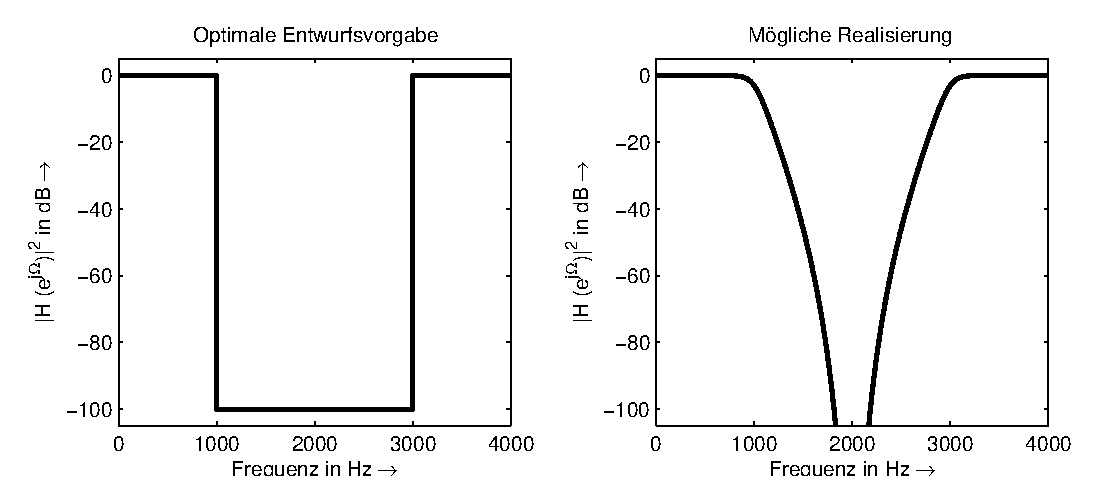
\includegraphics{psFilt/DesignBS}
    \caption{\label{pic:DesignBP}Optimaler Entwurf einer Bandsperre ($f_s$ = 8 kHz und
    Grenzfrequenz $f_1$ = 1 kHz und $f_2 = $ 3 kHz) und Realisierung durch Butterworth-Filter 6. Ordnung
    (siehe Abschnitt \ref{sec:Butterworth})}
    \end{center}
    \end{figure}
\end{itemize}

Eine weitere Gruppe von Filtern hat das Ziel Signale die durch
eine Übertragung verändert wurden, wieder in ihre ursprüngliche
Form zurück zu bringen. Das Ziel ist also, ein verändertes
Spektrum zu begradigen, bzw. auszugleichen. Aus dieser Aufgabe
folgt auch die verwendete englische Typbezeichnung Equalizer. In
der Tonstudiotechnik werden diese Filter zwar nicht nur zu diesem
Zweck verwendet, aber auch dort werden die Klangformungsfilter als
Equalizer bezeichnet. Equalizer ist ein sehr allgemeiner Begriff
und kann Filter beinhalten, die eine vollständige Vorgabe der
Übertragungsfunktion versuchen zu realisieren, zum Beipeil bei der
Hörgeräteanpassung, die eine vollständige Beschreibung des
Hörverlustes als Ausgangsbasis verwendet, oder aber es werden nur
bestimmte Bereiche verändert. Zu dieser letzten Gruppe gehören die
Equalizer, wie sie in der Tonstudiotechnik verwendet werden.
Hierbei unterscheiden wir zwischen den parametrischen Equalizern
und den sog. Terzband-Equalizer\footnote{Eine Terz beschreibt eine
drittel Oktave, die wiederum eine Frequenzverdoppelung
beschreibt.}.

Bei den parametrischen Equalizer können durch die drei Parameter
\begin{itemize}
    \item Frequenz,
    \item Verstärkung bzw. Abschwächung und
    \item Güte ($Q$-Faktor)
\end{itemize}
sehr genaue Eingriffe in das Klangspektrum vorgenommen werden.
Dabei ist die Güte $Q$ als Verhältnis von Mittenfrequenz und
Bandbreite definiert.
\begin{figure}[H]
\begin{minipage}{5cm}
%\begin{figure}[htb]
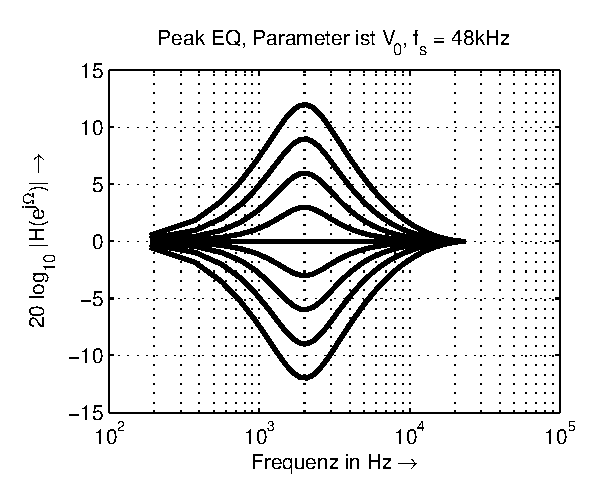
\includegraphics [width = 5cm]{psFilt/EQ_GainParam}
\caption{\label{pic:EQ_GainParam} Equalizerübertragungskurve bei Veränderung der Verstärkung}
%\end{figure}
\end{minipage}
\begin{minipage}{5cm}
%\begin{figure}[htb]
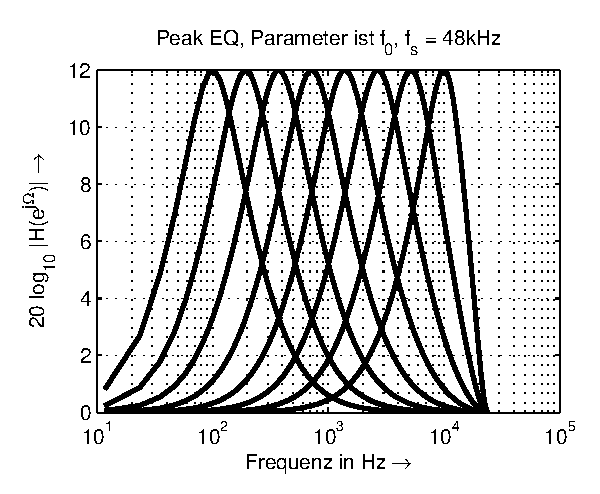
\includegraphics [width = 5cm]{psFilt/EQ_FreqParam}
\caption{\label{pic:EQ_FrequenzParam}Equalizerübertragungskurve bei Veränderung der Frequenz}
%\end{figure}
\end{minipage}
\begin{minipage}{5cm}
%\begin{figure}[htb]
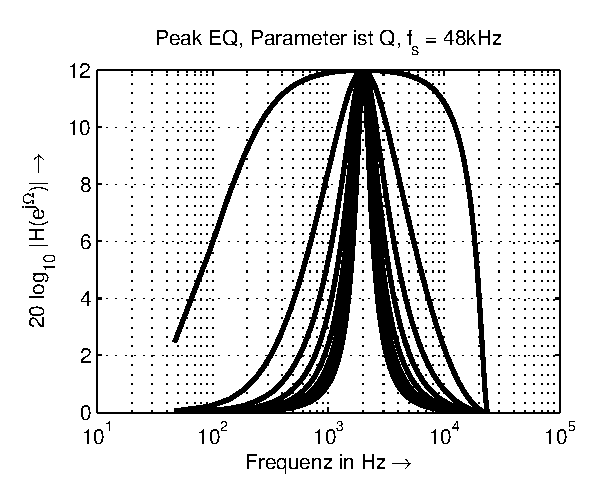
\includegraphics [width = 5cm]{psFilt/EQ_QParam}
\caption{\label{pic:EQ_GueteParam}Equalizerübertragungskurve bei Veränderung der Güte}
%\end{figure}
\end{minipage}
\end{figure}

Es gibt auch noch spezielle Filter für den Hoch- und
Tiefpassbereich, die als Kuhschwanzfilter (Shelving-Filter)
bezeichnet werden. Hierbei stehen nur die zwei Parameter Frequenz
und Verstärkung bzw. Abschwächung zur Verfügung.
\begin{minipage}{15cm}
\begin{figure}[H]
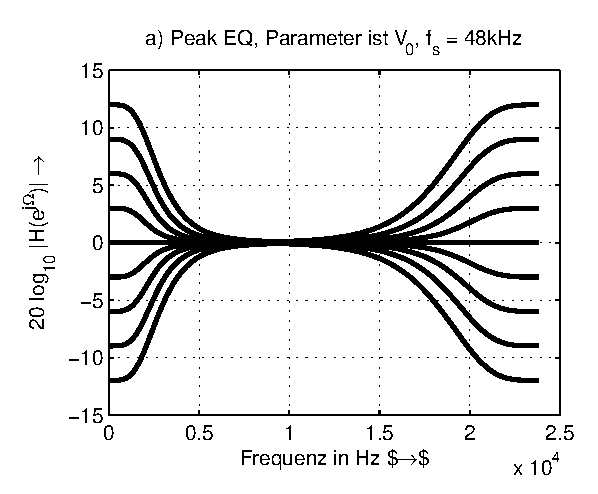
\includegraphics [width = 7cm]{psFilt/EQ_GainShelvParam}
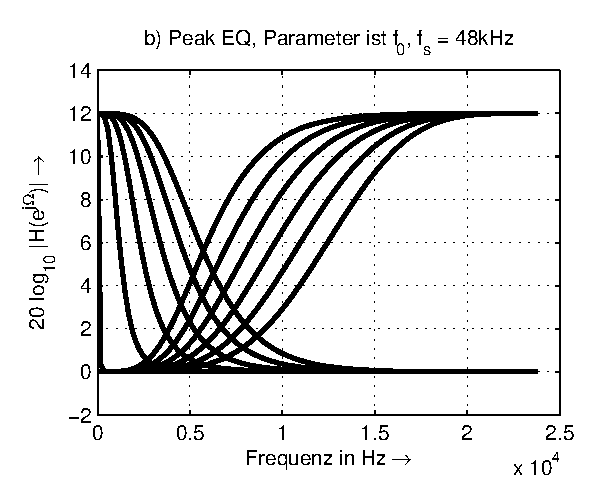
\includegraphics [width = 7cm]{psFilt/EQ_FreqShelvParam}
\caption{\label{pic:EQ_GainShelvParam} Equalizerübertragungskurve für einen
Hoch- und Tiefpasskuhschwanzfilter bei Veränderung der Verstärkung (a) und der Frequenz (b) }
\end{figure}
%\begin{figure}[H]
%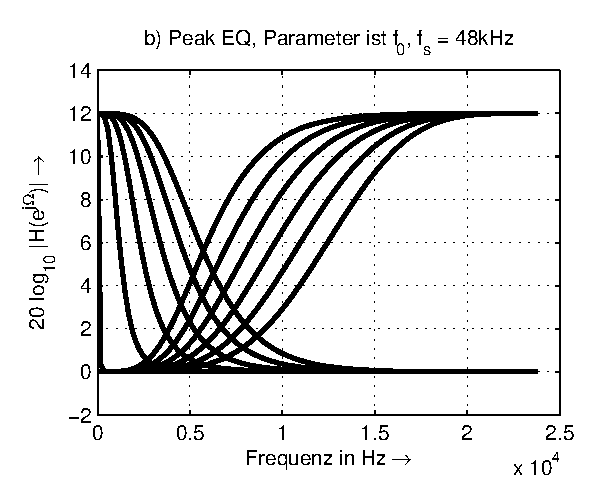
\includegraphics [width = 7cm]{psFilt/EQ_FreqShelvParam}
%\caption{\label{pic:EQ_FrequenzShelvParam}Equalizerübertragungskurve für einen
%Hoch- und Tiefpasskuhschwanzfilter bei Veränderung der Frequenz}
%\end{figure}
\end{minipage}


Im Gegensatz zu den vollparametrischen EQs sind bei
Terzband-Equalizer die Frequenzen und Güten festgelegt. Der Nutzer
hat nur einen Einfluss auf de Verstärkung oder Absenkung. Der
Vorteil dieser Equalizer ist ihre einfache Bedienung und die
Möglichkeit sofort zu sehen, welche Frequenzveränderungen
vorgenommen werden. Die Mittenfrequenzen der Filter sind
standardisiert. Tabelle \ref{Tab:MittenfrequenzenTerzband} gibt
diese Frequenzen wieder.
\begin{table}
\begin{tabular}{|c|c|c|c|}
  \hline
  % after \\: \hline or \cline{col1-col2} \cline{col3-col4} ...
  \multicolumn{2}{|c|}{Oktav-EQ}& \multicolumn{2}{|c|}{Terz-EQ}\\
\hline
  index & Frequenz (Hz) & index & Frequenz (Hz) \\
  \hline
     &      & -16 & 25 \\
  -5 & 31.5 & -15 & 31.5 \\
     &      & -14 & 40 \\\hline
     &      & -13 & 50 \\
  -4 & 63   & -12 & 63 \\
     &      & -11 & 80 \\\hline
     &      & -10 & 100 \\
  -3 & 125  & -9  & 125 \\
     &      & -8  & 160 \\\hline
     &      & -7  & 200 \\
  -2 & 250  & -6  & 250 \\
     &      & -5  & 315 \\\hline
     &      & -4  & 400 \\
  -1 & 500  & -3  & 500 \\
     &      & -2  & 630 \\\hline
     &      & -1  & 800 \\
  0  & 1000 & 0   & 1000 \\
     &      & 1   & 1250 \\\hline
     &      & 2   & 1600 \\
  1  & 2000 & 3   & 2000 \\
     &      & 4   & 2500 \\\hline
     &      & 5   & 3150 \\
  2  & 4000 & 6   & 4000 \\
     &      & 7   & 5000 \\\hline
     &      & 8   & 6300 \\
  3  & 8000 & 9   & 8000 \\
     &      & 10  & 10000 \\\hline
     &      & 11  & 12500 \\
  4 & 16000 & 12  & 16000 \\
    &       & 13  & 20000 \\
  \hline
\end{tabular}

\caption{\label{Tab:MittenfrequenzenTerzband}Mittenfrequenzen für
einen Terzband-Equalizer. Zusätzlich sind die Frequenzen für einen
Oktav-Equalizer angegeben.}
\end{table}

Für bestimmte Anwendungen (z.B. Synthesizer) werden auch manchmal
Filter verwendet, die in ihrer Grundcharakteristik den
Sperrfiltern entsprechen, aber zusätzlich in der Nähe der
Grenzfrequenz eine Verstärkung einbringen. Diese
Verstärkungsfrequenzen kommen bei natürlichen Musikinstrumenten
ebenfalls häufig vor. Man spricht in diesem Fall von sog.
Resonanzfrequenzen, da bestimmte Signalanteile im Filter eine
starke Resonanz finden.

\section{Realisierungsformen}
Wir haben gesehen, dass es eine Vielzahl von unterschiedlichen
Filtereinsatzmöglichkeiten gibt. Bisher wurde aber keinerlei
Hinweis auf die Realsierungsformen gegeben. Aus der Beschreibung
von Systemen kennen wir zwei unterschiedliche Systemarten. Die
Systeme mit Rückkopplung (rekursiv) und ohne. Als Bezeichnung
hatten wir eingeführt, Infinite Impulse Response (IIR) und Finite
Impulse Response (FIR) Systeme. Und genau diese Bezeichnungen
kennzeichnen auch die beiden grundsätzlichen Realisierungsformen
von Filtern.

\subsection{FIR-Filter}
Die Anwendung von FIR-Filtern ist ausschließlich durch digitale
Signalverarbeitung möglich, da eine Realisierung in Analogtechnk
mit elektrischen Bauelementen nicht möglich ist. FIR-Filter
zeichnen sich durch einige positive Eigenschaften aus. In erster
Linie kann die Stabilität immer garantiert werden. Alle FIR-Filter
sind stabil. Weiterhin ist es möglich mit FIR-Systeme Filter zu
realisieren, die nur den Betragsfrequenzgang verändern und sonst
nur eine zeitliche Verzögerung des Signals bewirken. Die zeitliche
Verzögerung macht sich in der Übertragungsfunktion durch eine
lineare Phase deutlich. Diese Filter werden deshalb linearphasig
genannt.

\subsubsection{Beschreibung als Blockdiagramm}
Bisher haben wir FIR-Systeme nur als Differenzengleichung
oder als
z-Übertragungsfunktion kennen gelernt. Um die noch folgende
Implementierung zu ermöglichen ist eine andere Darstellung aber
hilfreicher. Schaut man sich die Differenzengleichung für ein
FIR-Filter genauer an. So erkennt man, dass man 3 verschiedene
Bauteile braucht.
\begin{itemize}
    \item Addierer
    \item Multiplizierer
    \item Einen Verzogerungseinheit, die das Signal um genau einen
    Sample $T$ verzögert. Dies kann durch ein einfaches
    Speicherelement geschehen.
\end{itemize}
Diese 3 Elemente werden im folgenden durch die in Abbildung
\ref{pic:BlockDiagramSymbols} gezeigten Symbole beschrieben.

\begin{figure}[H]
\begin{center}
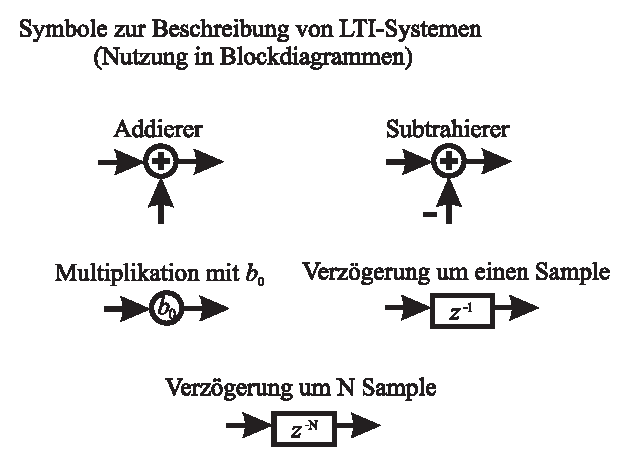
\includegraphics{psFilt/BlockdiagrammSymbole}
\caption{\label{pic:BlockDiagramSymbols}Symbole um Zeichnen von
Filter  Strukturen als Blockdiagramm}
\end{center}
\end{figure}

Beispielsweise ergibt sich für ein FIR-System erster Ordnung, dass
durch $y(k) = b_0 x(k) + b_1 x(k-1)$ beschrieben ist, das folgende
Blockschaltbild.
\begin{figure}[H]
\begin{center}
\includegraphics{psFilt/FIRErsterOrdnung}
\caption{\label{pic:FIRErsterOrdnung}Blockdiagramm eines
FIR-Filters 1. Ordnung}
\end{center}
\end{figure}

Zur Realisierung eines allgemeinen FIR-Filters muss das allgemeine
Blockschaltbild genauer betrachtet werden (siehe Abb. \ref{pic:FIR_Blockdiagramm}).
\begin{figure}[H]
\begin{center}
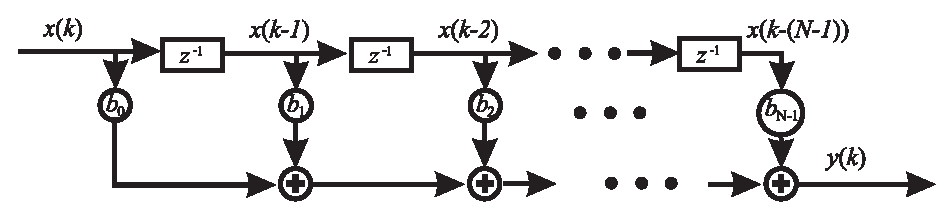
\includegraphics{psFilt/FIR_allgemeinBlock}
\caption{\label{pic:FIR_Blockdiagramm}Allgemeine FIR-Filter Struktur.}
\end{center}
\end{figure}

Es wird deutlich, dass wir bei $N$-Koeffizienten $N-1$
Speicherelemente benötigen, die die jeweilige Vergangenheit von
$x(k)$ speichern.

Um einen Ausgangswert $y(k)$ zu berechnen, muss die Summe
\begin{equation}\label{eq:FIR_Filter}
    y(k) = \sum_{i = 0}^{N-1} b_i x(k-i)
\end{equation}
berechnet werden. Abschließend wird der Speicher um eine Stelle
weiter geschoben. Gleichung \ref{eq:FIR_Filter} ist bereits von
der Faltung bekannt. Somit ist ein FIR-Filter also eine andere
Bezeichnung für ein System zur Faltung.

\subsection{FIR-Filter Design}
Nachdem die Strukturen zur Realisierung von Filtern bekannt sind, fehlt noch die Bestimmung
der einzelnen Filterkoeffizienten. Es muss also überlegt werden, wie aus einem bestimmten Entwurf
des Filters im Frequenzbereich, geeignete Koeffizienten im Zeitbereich berechnet werden können. Dazu betrachten
wir zunächst nur die FIR-Filter. Es sind verschiedene Verfahren bekannt. Die beiden am häufigsten
Methoden sollen im weiteren genauer erläutert werden.

\subsubsection{Fenster-Methode}
Aus dem Abschnitt über Spektren ist uns bekannt, dass wir zu einer Zeitfolge mit Hilfe der
DTFT ein Spektrum berechnen können, dass in $2\pi$ periodisch ist. Zu dieser Hintransformation gibt es
auch die korrespondierende Rücktransformation die als
\begin{equation}\label{FIR:IDTFT:Def}
    x(k) = \frac{1}{2\pi}\int_{-\pi}^{\pi} X\jom e^{j\Omega k} d\Omega
\end{equation}
definiert ist. Somit ist es natürlich auch möglich zu einem bestimmten Frequenzentwurf
eine zugehörige Zeitfolge zu berechnen.
Nehmen wir beispielsweise an, wir suchen die Koeffizienten, um ein ideales Tiefpassfilter mit der
Grenzfrequenz $\Omega_g$ zu realisieren. Die Definition der Übertragungsfunktion ist somit
\begin{equation}\label{FIR:BSP:Tiefpass}
    H\jom = \Bigg\{ \begin{array}{lcc}
1 & \fuer & -\Omega_g \leq \Omega \leq  \Omega_g\\
0 & & \Omega_g < |\Omega| \leq \pi
\end{array}
\end{equation}
Für die gesuchten Filterkoeffizienten ergibt sich
\begin{eqnarray}\label{FIR:TP:Ideal}
    h(k) & = &\frac{1}{2\pi}\int_{-\pi}^{\pi} H\jom e^{j\Omega k} d\Omega\\
         & = &\frac{1}{2\pi}\int_{-\Omega_g}^{\Omega_g}e^{j\Omega k} d\Omega\\
         & = &\frac{\Omega_g}{\pi} \frac{\sin(\Omega_g k)}{\Omega_g k}
\end{eqnarray}
Problematisch an diesem Ergebnis ist zum einen, dass sich die gefundene Koeffizienten
unendlich ausdehnen und zum anderen, dass das Filter auch noch nicht-kausale Anteile
enthält.
Aus dem ersten Grund muss immer eine Begrenzung vorgenommen werden. Das heißt die
gefundenen Koeffizienten werden nach einer
bestimmten Länge zu beiden Seiten der Zeitachse gleichmäßig abgeschnitten.
Dies führt nicht mehr zum idealen Tiefpass, sondern zu einer Approximation. Der sich
ergebende Fehler kann aus der Überlegung zur Spektrumsanalyse ersehen werden. Die Begrenzung
entspricht einer Gewichtung der Filterkoeffizienten mit einem Rechteck-Fenster.
Diese Multiplikation führt im Frequenzbereich zu einer Faltung mit der Übertragungsfunktion
des Rechtecks. Für den idealen Tiefpass hat das zwei Konsequenzen. Erstens ist der Übergang vom
Durchlass- zum Sperrbereich nicht mehr unendlich steil und zweitens enstehen an der Übergangsstelle
Überschwinger. Vergrößert man nun die Länge des Ausschnitts, so wird der Übergangsbereich schmaller,
und die Überschwinger konzentrieren sich an der Übergangsstelle, aber die Höhe der Überschwinger
bleiben gleich (siehe Abbildung \ref{pic:FIR:GippsBsp}). Dies wird als Gippsches Phänomen bezeichnet.
\begin{figure}[H]
\begin{center}
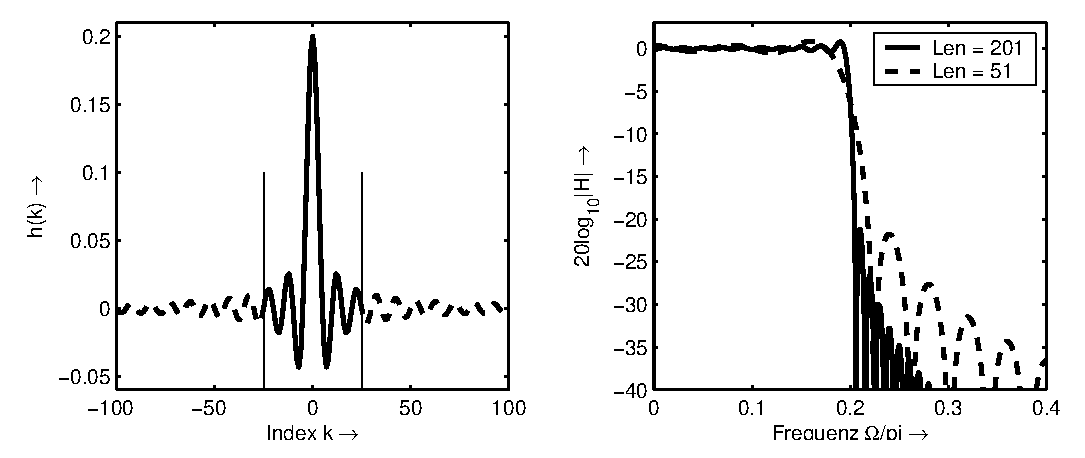
\includegraphics{psFilt/GippsPheanomen}
\caption{\label{pic:FIR:GippsBsp}Beispiel zur Veranschaulichung des Gipps-Phänomens}
\end{center}
\end{figure}

Die Ursache hierfür ist in der Übertragungsfunktion des Rechteckfensters zu suchen. Betrachtet
man diese Funktion für die beiden betrachteten Längen, so erkennt man die Konzenzentration der
Überschwinger bei der Frequenz Null. Die Höhe der Überschwinger bleibt aber identisch.
Genau dieses Verhalten wird durch die Faltung im Frequenzbereich auf die Übertragungsfunktion
des idealen Tiefpasses aufgeprägt. Man kann aber zeigen [KK98], dass die Approximation im
Sinne des kleinsten Fehlerquadrates {\em Minimum Mean Square Error (MMSE)} über
alle Frequenzen optimal ist.

Um die nicht-kausalen Anteile zu beseitigen ist zusätzlich noch eine zeitliche Verschiebung der
gefundenen Filterkoeffizienten notwendig. Diese Verschiebung führt dann, wie man durch den
Verschiebungssatz der Fourier-Transformation sieht, zu einer linearen Phase des entworfenen
Tiefpasses.

Zur Vermeidung der Überschwinger {\em Ripple} können nun dieselben Techniken verwendet werden, die auch die
Spektralanalyse verbessert haben. Eine Nutzung der dort vorgestellten Fensterfunktionen führt auf
eine geringere Ausprägung der Ripple, wobei gleichzeitig der Übergangsbereich zwischen
Durchgangs- und Sperrbereich zunimmt. Um das zu veranschaulichen, ist in Abbildung
\ref{pic:FIR:FensterEntwurf_1} der Entwurf eines Filters mit unterschiedlichen Fensterfunktionen
gezeigt. Man erkennt deutlich, dass mit zunehmendem Übergangsbereich die Überschwinger abnehmen, wobei
diese bei Nutzung der Fensterfunktionen nur noch im Sperrbereich deutlich zu erkennen sind.

\begin{figure}[H]
\begin{center}
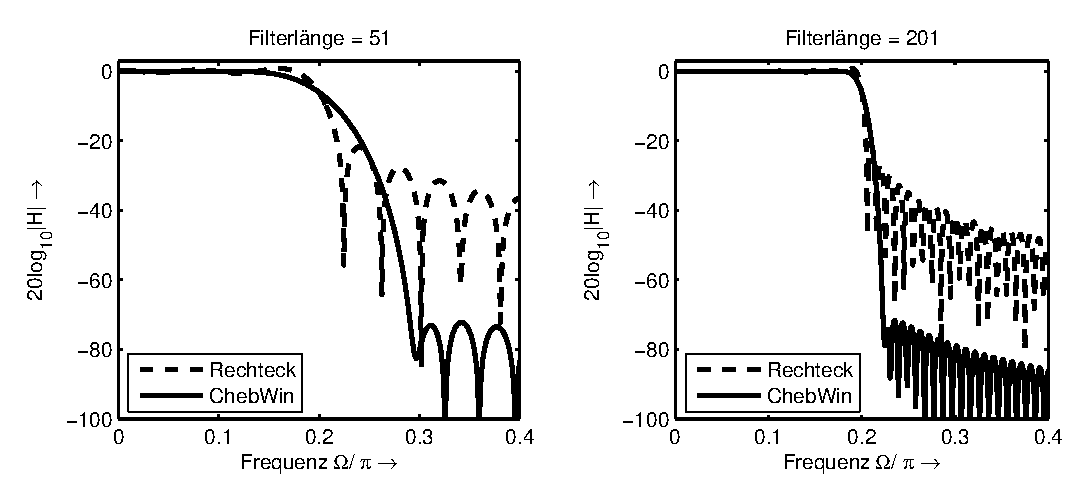
\includegraphics{psFilt/BspFensterEntwurf}
\caption{\label{pic:FIR:FensterEntwurf_1}Beispiel eines Tiefpass-Entwurfes mit Rechteck und Hann-Fesnster
unterschiedlicher Länge. Grenzfrequenz = $\Omega_g = 0.2\pi$}.
\end{center}
\end{figure}

\subsubsection{Parks-McClellan}
Im letzten Abschnitt wurde eine optimale Lösung vorgestellt, die den mittleren Fehler
über das Gesamtspektrum minimiert. Dabei hat sich aber der Fehler an der Übergangsstelle
konzentriert. Eine weitere optimale Lösung ist, den Fehler über alle Frequenzen gleich zu verteilen.
Die verbleibende Fehlergröße ist dabei nur von der gewählten Ordnung des Filters abhängig.
Zur Lösung dieses Problems wurde von Parks und McClellan der sog. Remez-Algorithmus entwickelt,
der zur optimalen Lösung konvergiert. Der Restfehler ist dabei minimal für alle Frequenzen.
Diese Minimierung des maximalen Fehlers wird auch als Tschebyscheff-Lösung bezeichnet.

Um die Lösung zu verdeutlichen und die Unterschiede zur Fenster-Methode heraus
zu arbeiten, ist in Abbildung \ref{pic:RemezVsFenster} ein Entwurf eines Tiefpass-Filters
mittels Remez-Entwurfsverfahren und mittels Fenster-Entwurfs mit Hann-Fenster gegenüber gestellt.
Wir erkennen, dass bei gleicher Ordnung das Remez-Verfahren eine insgesamt bessere Sperrdämpfung
zur Verfügung stellt. Dies bedeutet im Umkehrschluss, dass bei einer im Entwurf spezifizierten
Sperrdämpfung die Ordnung des resultierenden Filters beim Remez-Verfahren deutlich kleiner ist.
Für die konkrete Realisierung bedeutet dies eine deutliche Aufwandsreduktion.
\begin{figure}[H]
\begin{center}
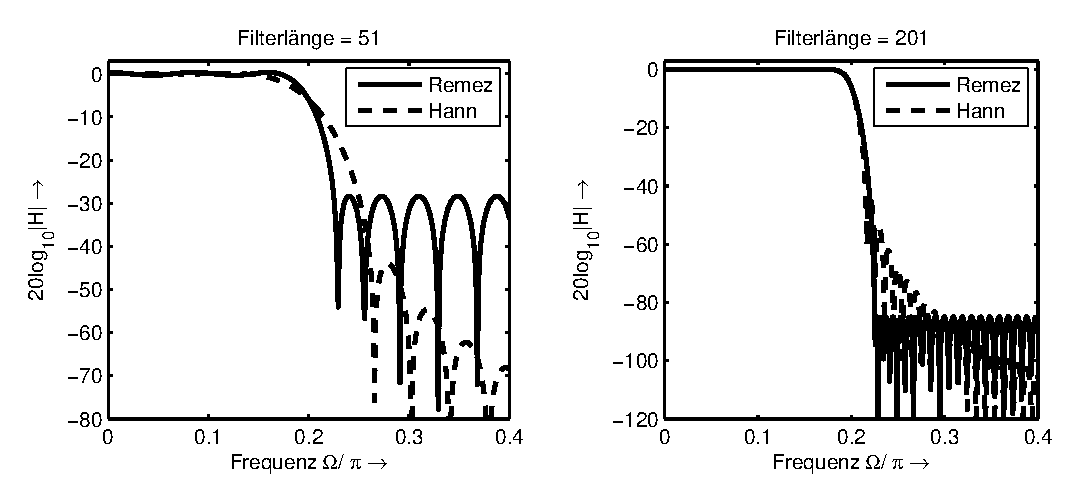
\includegraphics{psFilt/BspFensterRemez}
\caption{\label{pic:RemezVsFenster}Beispiel eines Tiefpass-Entwurfes mit dem Remez-Algorithmus
und der Fenster-Methode unterschiedlicher Länge. Grenzfrequenz = $\Omega_g = 0.2\pi$}.
\end{center}
\end{figure}

\tbd{Aufzeigen der Fenstermethode für allgemeine Übertragungsfunktionen,
Design im Frequenzbereich, IFFT und dann Ausschneiden, je nach Ordnung}


\subsubsection{Linearphasige Filter}
Linearphasigkeit ist eine interessante Eigenschaft in der Nachrichtentechnik,
da mit Ihrer Hilfe ein Signal gefiltert werden kann, ohne weitere Phasenverzerrungen
einzuführen. Weiterhin führt die Linearphasigkeit dazu, dass alle Frequenzanteile des
Signals um einen konstanten Betrag verzögert werden. Diese Verzögerung wird als
Gruppenlaufzeit bezeichnet und ist als Ableitung der Phase zur Frequenz definiert
\begin{equation}\label{eq:Def:Gruppenlaufzeit}
    \tau_g \jom = - \frac{\delta arg\{H \jom\}}{\delta \Omega}
\end{equation}

Wir haben bereits für das einfache Filter mit der Impulsantwort $h(k) = [1\:\: 1]$
festgestellt, dass es sich um einen Tiefpass mit linearer Phase handelt.
Diese Eigenschaft beruht drauf, dass die Nullstellen dieses FIR-Systems nur auf dem
Einheitskreis liegen. Zusätzlich sind aber auch alle Systeme linearphasig die am
Einheitskreis gespiegelte Nullstellen aufweisen. Es muss also gelten, dass
zu jeder Nullstellen die nicht auf dem Einheitskreis liegt $z_i$ eine weitere Nullstelle
mit $z_{\ell} = 1/z_i$ existiert.

Diese Symmetrie in der Pol-Nullstellenebene führt zu bestimmten Eigenschaften bei den
Koeffizienten. Man kann zeigen, dass 4 verschiedene Möglichkeiten existieren, linearphasige
FIR-Filter zu realisieren (KK98).
Diese unterscheiden sich darin, ob die Ordnung gerade oder ungerade ist und ob die Koeffizienten
zur Mitte des Filters achsen- oder punktsymmetrisch sind.
Daraus ergeben sich folgende Abhängigkeiten:

\begin{tabular}{|c|c|c|}
  \hline
  % after \\: \hline or \cline{col1-col2} \cline{col3-col4} ...
   & Achsensymmetrisch & Punktsymmetrisch \\
  \hline
  Gerade   & \parbox{7cm}{
\begin{center}
Typ I\\Es gilt $h(k) = h(M-k)$\\ mit $M$ als Filterordnung
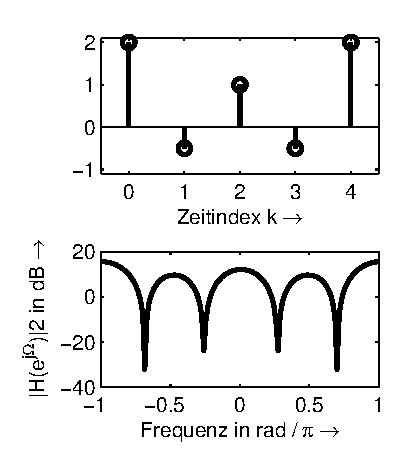
\includegraphics{psFilt/LinPhaseTypI}
Alle Filtercharakteristika möglich
\end{center}
} & \parbox{7cm}{
\begin{center}Typ II\\Es gilt $h(k) = -h(M-k)$ und\\
    $h(M/2) = 0$
\includegraphics{psFilt/LinPhaseTypII}
Nullstellen bei $\Omega = 0$ und $\Omega = \pm \pi$
\end{center}
} \\ \hline
  Ungerade & \parbox{7cm}{
\begin{center}Typ III\\kein Mittenkoeffizient\\Es gilt $h(k) = h(M-k)$
\includegraphics{psFilt/LinPhaseTypIII}
Nullstelle bei $\Omega = \pm \pi$
\end{center}
} & \parbox{7cm}{
\begin{center}Typ IV \\kein Mittenkoeffizient\\Es gilt $h(k) = -h(M-k)$
\includegraphics{psFilt/LinPhaseTypIV}
Nullstelle bei $\Omega = 0$
\end{center}
} \\
  \hline
\end{tabular}

Aus diesen vier Symmetrieanordnungen resultieren einige Eigenschaften für die Übertragungsfunktion.
Nur mit einem Filter Typ I lassen sich alle Grundfiltercharakteristika erzeugen. Bei den anderen Typen
ergeben sich feste Werte für bestimmte Punkte der Übertragungsfunktion. So ist für den Typ II immer eine
Nullstelle bei $\Omega = 0$ und $\Omega = \pi$, während der Typ III immer eine Nullstelle bei
$\Omega = \pm \pi$ besitzt. Typ IV  dagegen hat immer eine Nullstelle bei $\Omega = 0$

Dies hat natürlich Konsequenzen für den Entwurf von linearphasigen FIR-Filtern. So sollte man nie versuchen
einen Hochpass zu entwerfen und gleichzeitig Typ II oder Typ III verwenden wollen. Das heißt, man sollte
darauf achten, ob das gewünschte Filterverhalten, auch mit dem Entwurfsvorgaben zusammen passen.

\subsubsection{Minimalphasige FIR-Filter}
Eine weitere besondere Klasse an FIR-Filtern sind sogenannte minimalphasige Filter. Das heisst,
dieses Filter realisiert eine bestimmte Betragsübertragungsfunktion mit der minimalen Phase. Es zeigt
sich dass sich dieser Filtertyp genau dann ergibt, wenn alle Nullstellen innerhalb der Einheitskreises sind.
Eine Realisierung ist also entweder über ein Ausrechnen aller Nullstellen und deren Spiegelung
am Einheitskreis möglich, da sich so nur die Phase aber nicht das Betragsverhalten ändert. Der Aufwand zur
Zerlegung der Filter sehr hoher Ordnung ist numerisch aufwändig und nicht immer stabil durch
mögliche Rundungsfehler. Eine andere Methode nutzt die besondere Eigenschaft minimalphasiger Filter, dass es
eine direkte Verknüpfung zwischen dem Betrag und der Phase gibt. Hierzu wird die sog. Hilbert-Transformation
verwendet, die aber erst in einem späteren Abschnitt intensiver eingeführt wird. An dieser Stelle soll
ein Vorstellen des Design Algorithmus genügen, um eine beliebige Betragsübertragungsfunktion
(meist linearphasig, siehe Entwurfsmethoden) in einen minimalphasigen Entwurf zu überführen.
Gehen wir davon aus, dass die Betragsübertragungsfunktion $|H \jom|$ bekannt ist. Eine
Logarithmierung dieses Spektrums ist möglich, so lange keine echte Nullstelle vorhanden ist, dies
kann durch eine untere Schwelle gewährleistet werden. Dieses neue logarithmierte Spektrum wird
in den Zeitbereich mit Hilfe einer IDFT transformiert. Da es sich um eine reelle gerade Funktion
handelt, ergibt sich auch wieder eine reelle gerade Funktion. Diese Zeitbereichslösung wird nun
so verändert, dass alle negativen Zeiten (oder positive Zeiten oberhalb von N/2, durch die Zirkulareigenschaft
der DFT ist das gleichwertig) zu Null gesetzt werden und alle anderen Werte werden mit zwei multipliziert.
Diese neue Funktion wird nun mit der FFT erneut in den Frequenzbereich transformiert.
Um die Logarithmierung rückgängig zu machen wird für jeden Frequenzpunkt die Exponenten-Funktion angewendet.
Eine erneute IFFT der resultierenden Funktion führt auf die Filterkoeffizienten, die das minimalphasige
Filter repräsentieren.
Abbildung \ref{pic:MinimalphasigDesign} zeigt die Ergebnisse für
einen einfaches Filter achter Ordnung bei vorgegebenem Betragsübertragungsverhalten.
\begin{figure}[H]
\begin{center}
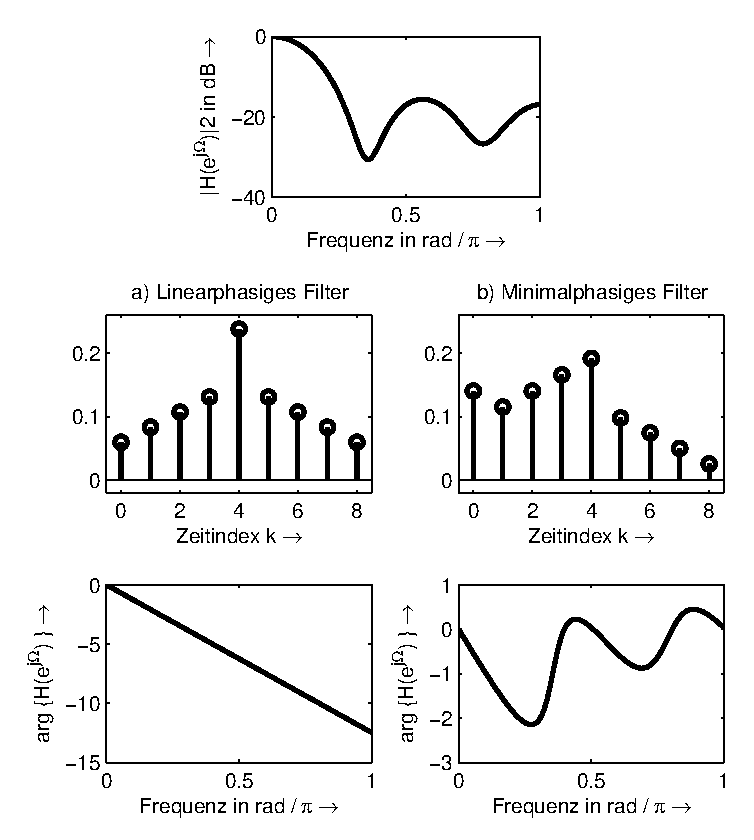
\includegraphics{psFilt/MinPhasenBsp}
\caption{\label{pic:MinimalphasigDesign}Entwurf eines Filters mit gegebener Betragsübertragungsfunktion. a)
als linearphasiges Filter und b) als minimalphasiges Filter.}
\end{center}
\end{figure}

Eine Matlab-Implementierung sehe folgendermaßen aus.
\begin{verbatim}
%v_H contains the magnitude vector of the desired filter
log_H = log(v_H+eps); % eps is the smallest positive number in matlab
                      % prevents log of zero
h_ceps = real(ifft(log_H)); % real for removing quantization error
h_ceps(2:length(h_ceps)/2) = 2*h_ceps(2:length(h_ceps)/2);
h_ceps(length(h_ceps)/2+1:end) = 0; % Setting to zero
H_min_log = fft(h_ceps);
H_min = exp(H_min_log);
v_h = real(ifft(H_min));
\end{verbatim}


\subsection{IIR-Filter}
Im Gegensatz zu den FIR-Filtern haben IIR-Filter auch rekursive Anteile. Die Implementierung
ist durch das Stabilitätsproblem sehr viel schwieriger. Gleichzeitig können sehr unterschiedliche
Strukturen verwendet werden, die alle unterschiedliche Eigenschaften haben.

\subsubsection{Beschreibung als Blockdiagramm}
Die Grundform des Blockdiagramms eines IIR-Filters ist in Abbildung \ref{pic:IIR_Blockdiagramm} gezeigt.

\begin{figure}[H]
\begin{center}
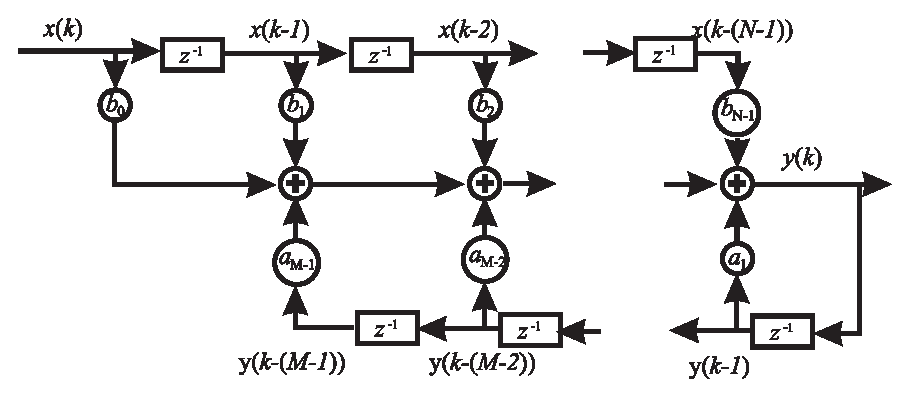
\includegraphics{psFilt/IIR_allgemeinBlock}
\caption{\label{pic:IIR_Blockdiagramm}IIR-Filter Struktur in Direkt Form I.}
\end{center}
\end{figure}

Diese sehr grundlegende Struktur, die die Differenzengleichung
geradlinig  umsetzt wird als Direkt Form I bezeichnet. Sie ist einfach in Matlab oder C++ umzusetzen.
Problematisch ist aber, dass bei einer höheren Ordnung $N>8$ numerische Probleme auftreten, da bei vielen
Filterentwürfen Filterkoeffizienten herauskommen, die im Zahlenbereich weit auseinander liegen und
schlecht gleichzeitig in einem quantisierten Datenformat repräsentiert werden können.

Um dies zu vermeiden, wird im allgemeinen eine Zerlegung von Filtern höherer Ordnung in Filter 2. Ordnung
vorgenommen. Diese werden dann {\em Second Order Sections} oder {\em Biquads} genannt. Eine kaskadierte
Schaltung führt dann abschließend wieder zum Originaldesign, ohne die numerischen Schwierigkeiten
zu beinhalten (siehe Abbildung \ref{pic:SOS_Zerlegung}).

\begin{figure}[H]
\begin{center}
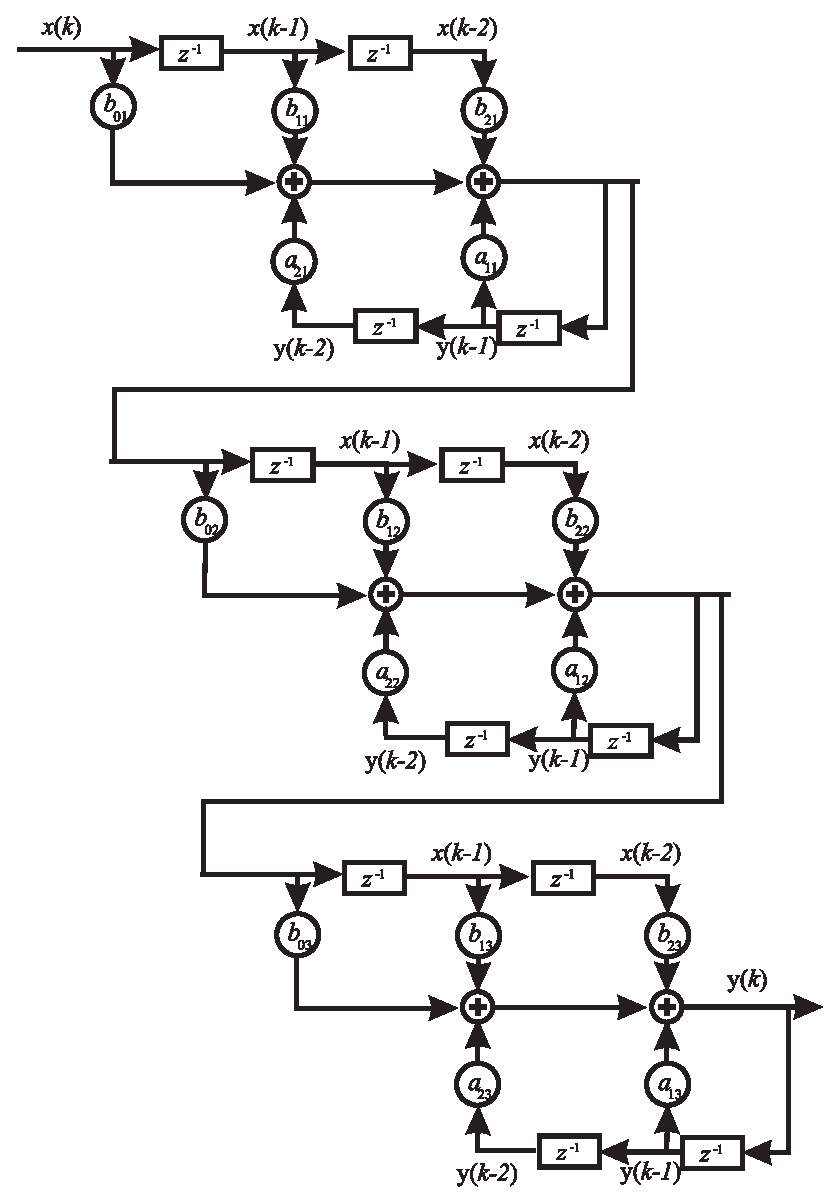
\includegraphics{psFilt/IIR_SOS_Zrlegung}
\caption{\label{pic:SOS_Zerlegung}Beispiel einer SOS-Zerlegung eines IIR-Filters 6.Ordnung.}
\end{center}
\end{figure}


Mathematisch lässt sich die Zerlegung folgendermaßen darstellen.
\begin{eqnarray}\label{eq:SOS:Zerlegung}
    H(z) &=& \frac{b_0 + b_1 z^{-1} +  b_2 z^{-2} + \cdots +  b_{N-1} z^{-(N-1)}}
                  {1 + a_1 z^{-1} +  a_2 z^{-2} + \cdots +  a_{N-1} z^{-(N-1)}} \\
         & = & \frac{b_{0_1} + b_{1_1} z^{-1} +  b_{2_1} z^{-2} }{1 + a_{1_1} z^{-1} + a_{2_1} z^{-2}}
         \frac{b_{0_2} + b_{1_2} z^{-1} +  b_{2_2} z^{-2} }{1 + a_{1_2} z^{-1} + a_{2_2} z^{-2}}  \cdots
         \frac{b_{0_N} + b_{1_N} z^{-1} +  b_{2_N} z^{-2} }{1 + a_{1_N} z^{-1} + a_{2_N} z^{-2}}
\end{eqnarray}
Die Zusammenführung zweier Pole und Nullstellen sollte dabei immer so erfolgen, dass die Pole
und Nullstellen möglichst dicht beieinander liegen (siehe Abbildung \ref{pic:SOS_ZerlegungZEbene}).

\begin{figure}[H]
\begin{center}
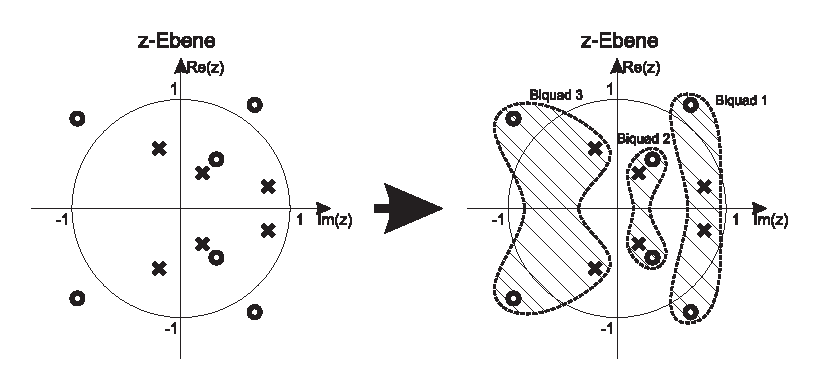
\includegraphics{psFilt/Zp2sos}
\caption{\label{pic:SOS_ZerlegungZEbene}Pol-Nullstellenzuordnung eines Filters 6.Ordnung zu
drei Second Order Sections.}
\end{center}
\end{figure}

\subsubsection{Filterstrukturen für SOS}
Die Direkt Form I ist nicht die einzige Möglichkeit ein IIR-Filter zu realisieren. Um die anderen
Strukturen zu verdeutlichen, konzentrieren wir uns auf die wichtigen SOS-Filter. Eine wichtige
Anforderung an Realisierungen spielen die Anzahl der Multiplikationen und die Anzahl der benötigten
Speicherplätze. Zusätzlich muss noch auf das numerische Verhalten bei einer quantisierten
Datendarstellung geachtet werden. Den letzten Punkt werden wir zunächst nicht behandeln.

Eine Analyse der DF1 zeigt, dass wir fünf Multiplikationen und vier Speicherplätze benötigen.
Durch Umstellen des Blockdiagramms lässt sich erkennen, dass es möglich ist die Speicher
für den Transversal- und für den Rückführungszweig zusammen zu legen (siehe Abbildung \ref{pic:IIR:DF1toDFII}).
Diese Umstellung ist erlaubt, da wir zum einen den Transversal- und den Rückführungszweig als zwei getrennte
Systeme auffassen können, zum anderen da beide Einzelsysteme LTI-Systeme sind und somit
das Vertauschen keinen Einfluss auf das Übertragungsverhalten hat. Die jetzt parallel liegenden
Speicherelemente können in einem abschließenden Schritt zusammen gefasst werden.
Es ergibt sich die sogenannte Direkt-Form II mit einer minimalen Anzahl von zwei Speicherelementen.
Strukturen mit minimaler Anzahl an Speicherelementen werden kanonisch genannt.

\begin{figure}[H]
\begin{center}
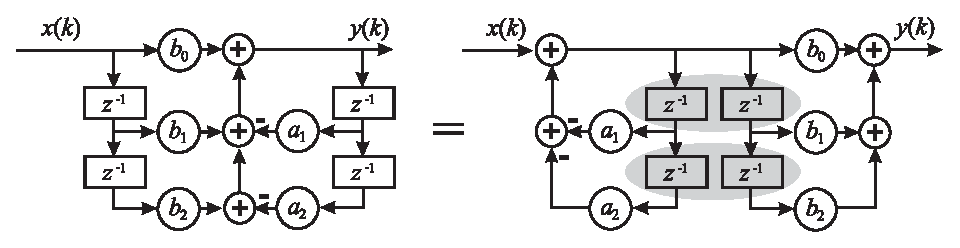
\includegraphics{psFilt/DF1_to_DF2}
\caption{\label{pic:IIR:DF1toDFII}Umwandlung einer DF1 Struktur in
die kanonische DF2 Struktur. Die grau hinterlegten
Verzögerungselemente können zu einem Element zusammen gefasst
werden, da sie jeweils dasselbe Signal als Eingang haben.}
\end{center}
\end{figure}

%Zusätzlich gibt es auch noch die kanonische Direkt Form III, die durch Umstellung der DFII erreicht wird.
%\tbdb{Umstellung von DF2 zu DF3}
\subsubsection{Vom Blockdiagramm zur Übertragungsfunktion}
\tbd{Analyse des Block-Diagramms mit z-Trafo daraus folgend die Übertragungsfunktion ,
??Wie geht es anders herum??}

\subsection{IIR-Filterdesign}
Um die Theorie des Entwurfs traditioneller IIR-Filter genauer zu erläutern fehlen an dieser Stelle noch
einige theoretische Konzepte. Der noch folgende Abschnitt \ref{sec:Analog}
zeigt die notwendigen Entwurfsverfahren.
Ein erster Einblick, um bereits mit IIR-Filtern arbeiten zu können,
wird in Abschnitt \ref{sec:MatlabFilter} auf Basis von Matlab gegeben.

Mit den bisherigen Erkenntnissen sind aber schon Lösungen für einige spezielle Filter
möglich.
\subsubsection{Notch-Filter}
\tbd{Entwurf in z-Ebene durch Nullstellen auf dem Einheitskreis und Polstellen mit verringertem
Radius und gleichem Winkel, Anwendungen bzw. Design Bsp.: DC Filter, Netzbrummfilter}
\subsubsection{Allpässe}
\tbd{Wiederholung spezielles Pol-Nullstellendiagramm, Überlegungen zum Entwurf im z-Bereich,
Anwendungen: Spezielle Filter}

\section{Implementierungsaspekte}
\subsection{FIR-Filter}
\subsubsection{Schnelle Faltung OLA}
Das Hauptproblem der FIR-Filter ist das beim Entwurf meist sehr hohe Filterordnungen mit mehr als
100 Koeffizienten herauskommen. Dies führt zu einer sehr hohen Rechenleistung, wenn man versucht solche
Filter direkt durch die Faltungssumme zu realisieren. Statt dessen kann eine FFT basierte schnelle
Faltung aufgebaut werden, die eine sehr viel recheneffizientere Version ermöglicht.

Wir hatten im Abschnitt (\ref{sec:DFT:Faltung}) gesehen, dass bei der Faltung mit Hilfe der FFT unbedingt genügend
Nullen angefügt werden müssen, um die zirkulare Faltung zu verhindern.
Für den Fall, dass die beiden Folgen eine sehr unterschiedliche Länge haben und dies
ist der Normalfall kommen weitere Probleme hinzu. Zum einen müssen riesige Speicherblöcke
angelegt werden, um die Signale zu speichern und zum anderen kann die Berechnung erst statt finden,
wenn alle Werte eingelesen sind. Da die FFT Größen zusätzlich auch noch für die Multiplikation der beiden
Spektren gleich lang sein müssen, bedeutet dies auch, dass man sehr viele unnötig angehängte Nullen
des Koeffizientenvektors ebenfalls transformieren muss.

Zur Lösung dieses Problems wird die Linearität der FFT ausgenutzt. Es ist möglich das Eingangssignal
in kleinere Blöcke zu zerlegen, die so lang gewählt werden, dass sie zu der Anzahl der
Filterkoeffizienten passt. Diese kleineren Blöcke werden mit Nullen so verlängert, dass die zirkulare
Faltung verhindert wird. Nimmt man an, dass das Filter die Ordnung $M$ hat und die Zerlegung
der Eingangsfolge in Blöcken der Länge $L$ vorgenommen wird, so ergibt sich die Länge der
Ausgangsfolge\footnote{Die Ordnung ist $M$, somit hat das Filter $M+1$ Koeffizienten, die Faltung ergibt dann
$L+M+1-1$ Ausgangswerte.} als $L+M$. Möchte man dieses Ergebnis mit Hilfe der FFT erreichen, muss
also der Eingangsblock um $M$ Nullen erweitert werden ({\em Zero-Padding}). Die benötigte
FFT-Größe ergibt sich dann aus der folgenden Zweier-Potenz von $L+M$. Das Ergebnis der Multiplikation
der Spektren des Filters mit dem der Eingangsfolge wird anschließend in den Zeitbereich zurück transformiert.
Dabei entsteht eine Zeitfolge der Länge $L+M$. Um nun für eine in Blöcken zerlegte Eingangsfolge
genau das Ausgangssignal einer direkten Faltung zu erhalten, muss nun das Ausgangssignal
des nächsten Blockes zu den $M$ überhängenden Ausgangswerten hinzu addiert werden. Da es sich hierbei
um eine Überlappung handelt, wird dieses Verfahren als {\em Overlap-Add} (OLA) bezeichnet.
Zur Verdeutlichung ist der gesamte Aufbau auch noch in Abbildung \ref{pic:OLA:Erklaerung} gezeigt.

\begin{figure}[H]
\begin{center}
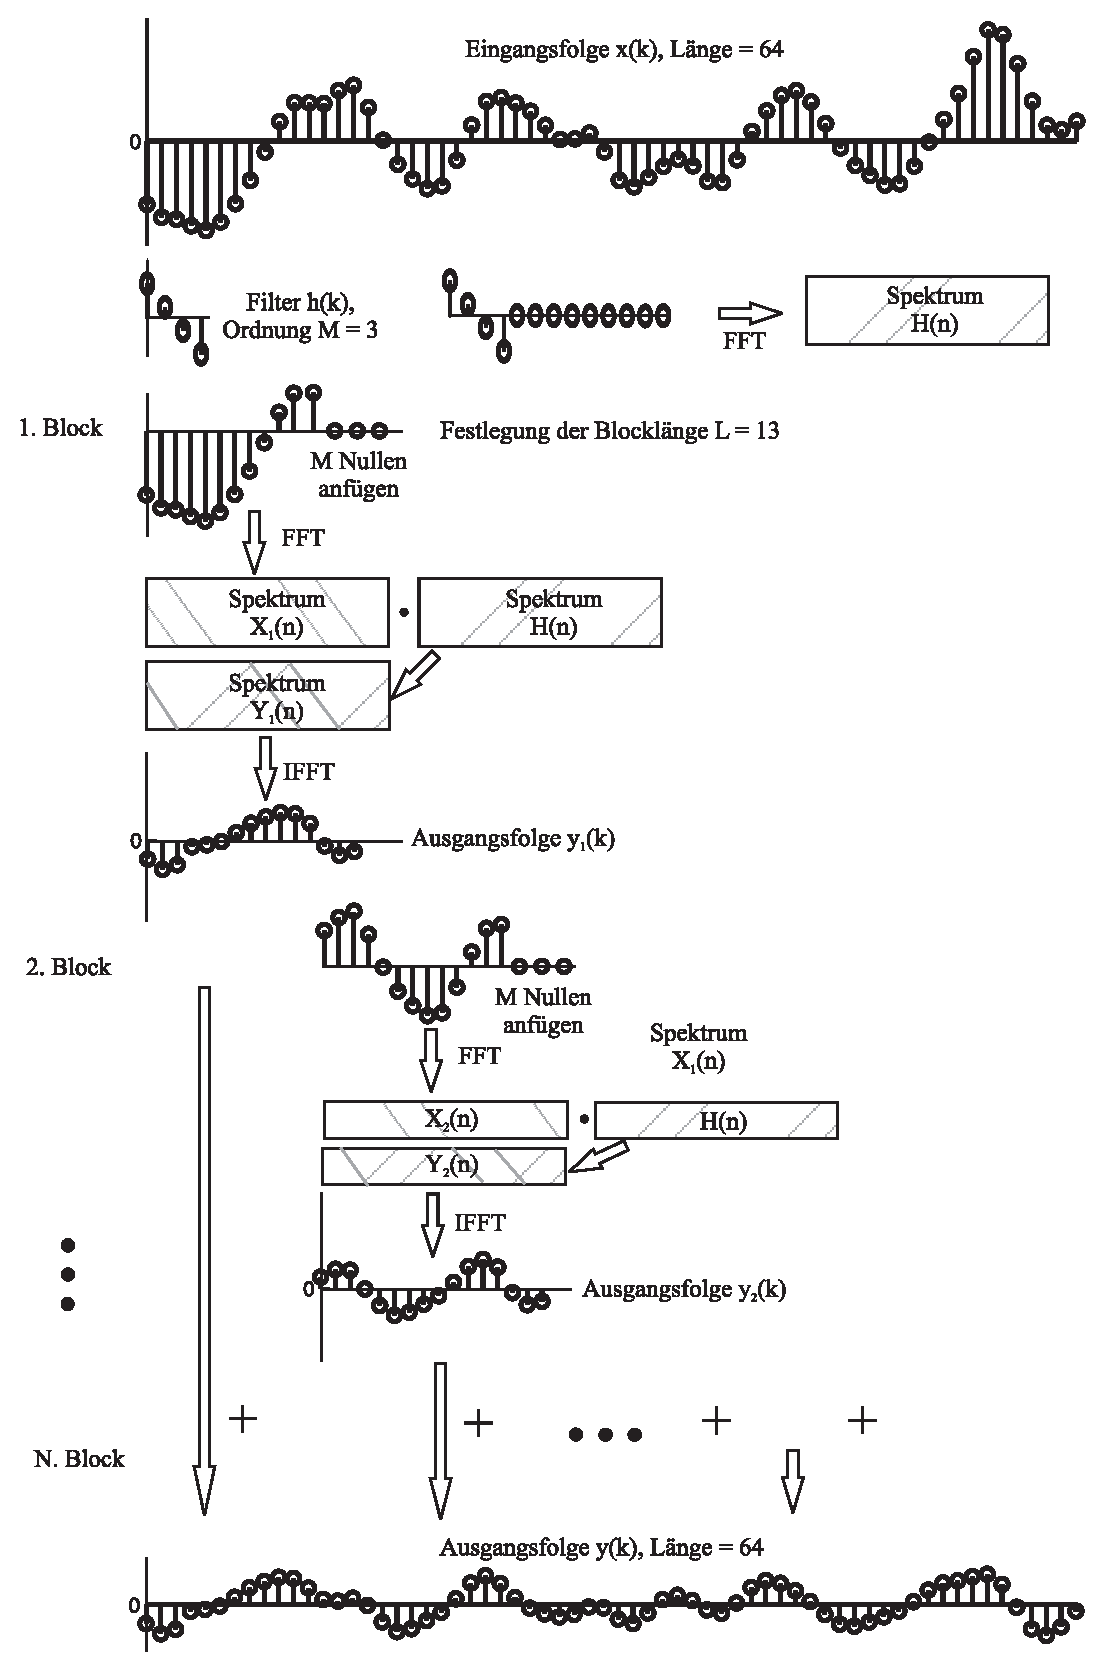
\includegraphics[width = 15cm]{psFilt/OLA_Erklaerung}
\caption{\label{pic:OLA:Erklaerung}Overlap-Add Verfahren am Beispiel mit $M = 3$ und $L = 13$.}
\end{center}
\end{figure}

Dieses Prinzip kann zusätzlich auch für sehr lange Impulsantworten, wie sie bei raumakustischen
Messungen vorkommen nützlich sein. In diesem Fall wird nicht nur das Eingangssignal, sondern auch
die Impulsantwort in kleine Blöcke zerlegt. Durch eine geeignete Struktur mit Verzögerungen der
einzelnen Spektren lässt sich so eine schnelle Faltung mit einer kurzen Latenz
(Durchlaufzeit) erzeugen. Dieses Verfahren wird Block Partitionierte OLA genannt und
ist insbesondere zur Realisierung von Faltungshallalgorithmen in kommerziellen Produkten erhältlich.

\subsubsection{C/C++}
Um die Umsetzung auf programmierbaren Systemen zu erläutern,
werden im weiteren Verlauf hauptsächlich Beispiele in C/C++ bzw.
Matlab verwendet.

Eine direkte C-Implementierung der Hauptroutine des FIR-Filters
ist durch den folgendes Programm gegeben. Wir gehen davon aus,
dass der Speicher für die vergangenen Werte und die Koeffizienten
ordnungsgemäß allokiert wurden. Als Eingangssignal wird ein Block
von Samples angenommen, der in In gespeichert ist.
\begin{verbatim}
for(kk = 0 ; kk < LenOfInput ; kk++)
{
    // Zuweisung des Aktuellen Samples
    bStates[0] = In[kk];

    // Berechnung der Summe (Zum besseren Vergleich
    // mit zweiter Methode, erster Koeffizient separat)
    Out[kk] = bCoeffs[0] * bStates[0];

    int nn;
    for (nn = 1 ; nn < LenOfFilter ; nn++)
    {
        Out[kk] += bCoeffs[nn] * bStates[nn];
    }
    // Verschieben der States
    // muss von hinten nach vorne erfolgen, damit der Speicher
    // nicht ueberschrieben wird
    for (nn = LenOfFilter-1 ; nn > 0 ; nn--)
    {
        bStates[nn] = bStates[nn-1];
    }
}
\end{verbatim}

Diese Version kann durch eine sehr viel schnellere Lösung ersetzt werden, wenn das
Konzept des Ringspeichers eingeführt wird, den es zwar bei spezialisierten digitalen Signal
Prozessoren (DSP) gibt, der aber in allgemeineren Rechnerarchitekturen (PC) nicht direkt vorkommt. Es
ist aber möglich eine Simulation dieses Speichers aufzubauen, um so eine effizientere
Implementierung zu ermöglichen.

Das Konzept des Ringspeichers geht davon aus, dass Speicher nicht linear sondern zirkular
aufgebaut ist. Dies wird in DSPs durch eine spezielle Modulo-Adressierung erreicht.
Abbildung \ref{pic:ZirkularMemeory} zeigt, wie man sich diesem Speicher vorstellen kann.
Ein neuer Datenwert wird immer an die Adresse geschrieben, auf die der rotierende Zeiger zeigt.

\begin{figure}[H]
\begin{center}
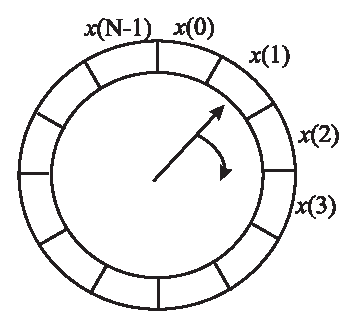
\includegraphics{psFilt/RingspeicherMemeory}
\caption{\label{pic:ZirkularMemeory} Schematische Darstellung eines Ringspeichers mit rotierndem
Adresszeiger}
\end{center}
\end{figure}

Eine Realiserung in C würde den Sprung am Übergang von $x(N-1)$
auf $x(0)$ durch eine if-Abfrage lösen. Diese Art der
Implementierung ermöglicht es ein FIR-Filter aufzubauen, dass ohne
Speicherverschiebung auskommt.

\begin{verbatim}
int ActPosStates = 0;
int nn;
for(kk = 0 ; kk < LenOfInput ; kk++)
{
    // Zuweisung des Aktuellen Samples
    bStates[ActPosStates] = In[kk];

    // Zuweisung des ersten Coeffs
    Out[kk] = bCoeffs[0] * bStates[ActPosStates];

    for (nn = 1 ; nn < LenOfFilter ; nn++)
    {
        ActPosStates--; // States zaehlen runter
        if (ActPosStates<0) // Falls Grenze erreicht
            ActPosStates+=LenOfFilter;  // Sprung ans Ende
        Out[kk] += bCoeffs[nn] * bStates[ActPosStates]; // Summe
    }
}
\end{verbatim}

Diese Lösung kann noch weiter optimiert werden, in dem der Sprung des Filters vorher berechnet wird.
Die if-Abfrage kann somit ebenfalls aus der Schleife entfernt werden. Zusätzlich ist es noch nützlich
pre-increment zu verwenden, da dies schneller abgearbeitet werden kann (Bartning-Script).

Der optimierte Code eines FIR-Filters lautet also.

\begin{verbatim}
int ActPosStates = 0;
int nn;
int Jump;

for(kk = 0 ; kk < LenOfInput ; ++kk)
{
    // Zuweisung des Aktuellen Samples
    bStates[ActPosStates] = In[kk];

    // Zuweisung des ersten Coeffs
    Out[kk] = 0;

    Jump = ActPosStates; // Jump Point

    for (nn = 0 ; nn <= Jump ; ++nn) //preincrement is faster
    {
        Out[kk] += bCoeffs[nn] * bStates[ActPosStates]; // Summe
        --ActPosStates; // States zaehlen runter
    }

    ActPosStates+=LenOfFilter;  // Sprung ans Ende

    Jump++;

    for (nn = Jump ; nn < LenOfFilter ; ++nn) //preincrement is faster
    {
        Out[kk] += bCoeffs[nn] * bStates[ActPosStates]; // Summe
        --ActPosStates; // States zaehlen runter
    }

    ActPosStates++;

    if (ActPosStates==LenOfFilter)
        ActPosStates -= LenOfFilter;

}

\end{verbatim}

Welche der beiden letzten Versionen schneller ist, hängt vom
Prozessortyp, von der Filterlänge und vom Compiler ab. Es hilft
also beim Entwickeln von zeitkritischen Routinen immer nur der
wirkliche Benchmark-Test unter realistischen Bedingungen.

\subsubsection{Vektorielle Schreibweise und Implementierung (Matlab)}
Häufig ist es nützlich, Signale als Vektoren aufzufassen, da durch die Vektor und
Matrix-Schreibweise bestimmte Rechenregeln und Eigenschaften der linearen Algebra
direkt für Signale nutzbar sind. Als Schreibweise werden meist fettgedruckte
Buchstaben verwendet. Typischerweise werden Zeitsignale als Spaltenvektoren eingeführt.

Beispiel eines Vektors mit vier vergangenen Zeitwerten
\begin{equation}\label{eq:DefSpaltenvektor}
    \vek{x}(k) = \left(%
\begin{array}{c}
  x(k) \\
  x(k-1) \\
  x(k-2) \\
  x(k-3) \\
\end{array}%
\right)
\end{equation}

Führen wir nun in der selben Art einen Vektor für die Koeffizienten ein
\begin{equation}\label{ed:Def:KoeffVektor}
    \vek{b} = \left(%
\begin{array}{c}
  b_0 \\
  b_1 \\
  b_2 \\
  b_3 \\
\end{array}%
\right),
\end{equation}
so kann der Ausgang $y(k)$ durch das Skalarprodukt dieser beiden Vektoren
ausgedrückt werden.
\begin{equation}\label{eq:FIR:VEk}
    y(k) = \vek{x}^T(k) \vek(b),
\end{equation}
wobei $^T$, die Transponierung bezeichnet. Für komplexe Signale würde man statt dessen die konjugiert
komplexe Transponierung verwenden, die als hermitescher Operator $^H$ bekannt ist.

Da Matlab vektoriell orientiert ist, lässt sich ein FIR-Filter besonders effizient implementieren, wenn
man nicht auf die internen Filter-Routinen zurückgreifen möchte.

\begin{verbatim}
v_states = zeros(LengthOfFilter,1);

for kk = 1:length(InputVektor)         % Annahme Daten stehen in InputVektor
  v_states(1) = InputVektor(kk);       % Neuen Datenwert in State speichern
  out(kk) = v_Coeffs.' * v_states;     % Skalarprodukt berechnen
  v_states(2:end) = v_states(1:end-1); % State Vector verschieben
end
\end{verbatim}

\subsection{IIR-Filter}

\subsubsection{IIR-Filterdesign\label{sec:MatlabFilter}}
Der Entwurf von IIR-Filtern erfolgt historisch bedingt etwas anders. Rekursive Filter
sind sehr viel enger mit analogen Filtern verwandt. Eine Möglichkeit des IIR-Filterentwurfs
besteht deshalb darin, einen analogen Entwurf durchzuführen und das Resultat in den Digitalbereich
zu transformieren. Da bisher noch keine analogen Filter genauer besprochen wurden, soll an dieser Stelle
nur Beispielhaft typische Lösungen und ihre Stärken und Schwächen gezeigt werden.

\subsubsection{Butterworth-Filter}
Ziel des Butterworth-Entwurfs ist einen möglichst flachen Durchlassbereich zu erhalten.
Dies wird im analogen Entwurf durch Nutzung einer Potenzfunktion gewährleistet (siehe Abschnitt Analogentwurf)
Aus diesem Grund wird dieser Entwurf auch als {\em Maximum Flat Design} bezeichnet.
In Matlab stehen die Befehle \verb+butter+ und \verb+buttord+ für das Design zu Verfügung, wobei
mit buttord zu einem definierten Design die benötigten Entwurfsparameter bestimmt werden und
butter der eigentliche Entwurf ist. Angegeben werden meist zwei Arbeitspunkte des Filters, zum einen
bis zu welcher Frequenz der Durchlassbereich definiert ist und welche Abstand von der 0dB Linie noch als
Durchlass gilt. Zum anderen ab welcher Frequenz eine bestimmte Dämpfung erreicht werden muss (Sperrbereich).
Da die Grenzfrequenz des Butterworth-Filter durch die $-3$dB Grenze definiert, wird in Butterord eine
Anpassung an diese Frequenz vorgenommen.

Beispiel einer Filterspezifikation für normierte Frequenzen:\\
Durchlassbereich bis $0.1\pi$ und maximale Dämpfung von $0.2$dB.\\
Sperrbereich ab $02\pi$ und minimale Dämpfung von $30dB$.\\
Der dazugehörige Matlab-Code sieht dann wie folgt aus:

\begin{verbatim}
Pass_freq = 0.1; % Matlab uses normalized frequencies from 0..2
Pass_dB = 0.2;
Stop_freq = 0.2;
Stop_dB = 30;

[N,f_g] = buttord(Pass_freq,Stop_freq,Pass_dB,Stop_dB);
% Result is 7th Order and f_g = 0.1247
[b,a] = butter(N,f_g);
\end{verbatim}

\subsubsection{Tschebyscheff-I-Filter}
Im Gegensatz zum Butterworth-Filter ist das Ziel des Tschebyscheff-I Filters
im Durchlassbereich die maximal zulässige Durchlassdämpfung nicht zu überschreiten. Gleichzeitig
wird aber erlaubt, diesen Bereich bis zur Grenzfrequenz auszunutzen. Die Tschebyscheff-Optimierung
hat also immer zum Ziel den Maximalen Fehler zu minimieren. Der Entwurf wird
auch als Equiripple-Design bezeichnet.
Dies führt zu einem Entwurf mit geringerer Ordnung. Die zugehörigen Matlab-Befehle lauten
\verb+cheb1ord+ und \verb+cheby1+. Für das Design-Beispiel ergibt sich der folgende
Matlab-Code.

\begin{verbatim}
Pass_freq = 0.1; % Matlab uses normalized frequencies from 0..2
Pass_dB = 0.2;
Stop_freq = 0.2;
Stop_dB = 30;

[N,f_g] = cheb1ord(Pass_freq,Stop_freq,Pass_dB,Stop_dB);
% Results in a 5th Order filter with f_g = 0.1
[b,a] = cheby1(N,Pass_dB,f_g);
\end{verbatim}

\subsubsection{Tschebyscheff-II-Filter}
Das Tschebyscheff-II-Filter ist der Inverse Entwurf zum Typ I. Das Ziel ist also ein
flacher Durchlassbereich und ein oszilierender Sperrbereich.
Der dazugehörige Matlab-Code sieht folgendermaßen aus.

\begin{verbatim}
Pass_freq = 0.1; % Matlab uses normalized frequencies from 0..2
Pass_dB = 0.2;
Stop_freq = 0.2;
Stop_dB = 30;

[N,f_g] = cheb2ord(Pass_freq,Stop_freq,Pass_dB,Stop_dB);
% Results in a 5th Order filter with f_g = 0.2
[b,a] = cheby2(N,Stop_dB,f_g);
\end{verbatim}

\subsubsection{Cauer-Filter}
Das Cauer-Filter auch als Ellpitisches-Filter bezeichnet, definiert einen
Equiripple-Entwurf im Durchlass- und Sperrbereich. Dies führt zu einer weiteren
Reduzierung der Ordnung. Der Matlab-Entwurf sieht wie folgt aus.
\begin{verbatim}
Pass_freq = 0.1; % Matlab uses normalized frequencies from 0..2
Pass_dB = 0.2;
Stop_freq = 0.2;
Stop_dB = 30;

[N,f_g] = ellipord(Pass_freq,Stop_freq,Pass_dB,Stop_dB);
% Results in a 4th Order filter with f_g = 0.1
[b,a] = ellip(N,Pass_dB,Stop_dB,f_g);
\end{verbatim}

\subsubsection{Vor- und Nachteile der unterschiedlichen Entwurfsverfahren}

Die Wahl der Entwurfsmethode beruht im großen Maße auf den gegebenen Randparamtern. Um eine geeignete
Wahl zu treffen ist es aber notwendig die Stärken und Schwächen der einzelnen Verfahren zu beleuchten.
Aus den vorherigen Abschnitten ist bereits ersichtlich, dass die Ordnung der Filter und somit die Anzahl der
benötigten Filterkoeffizienten vom Entwurf abhängt. Der Butterworth-Entwurf benötigt immer die größte
Ordnung, während das Cauer-Filter immer mit der geringsten Ordnung auskommt. Gleichzeitig sind die
resultierenden Koeffizienten auch für eine SOS-Lösung numerisch am fragilsten und benötigen eine hohe
Quantisierung.

Um die weiteren Vor- und Nachteile zu verdeutlichen sind in Abbildung \ref{pic:IIR:DesignBsp} die
verschiedenen Entwurfsverfahren am oben verwendeten Beispiel gezeigt.
\begin{figure}[H]
\begin{center}
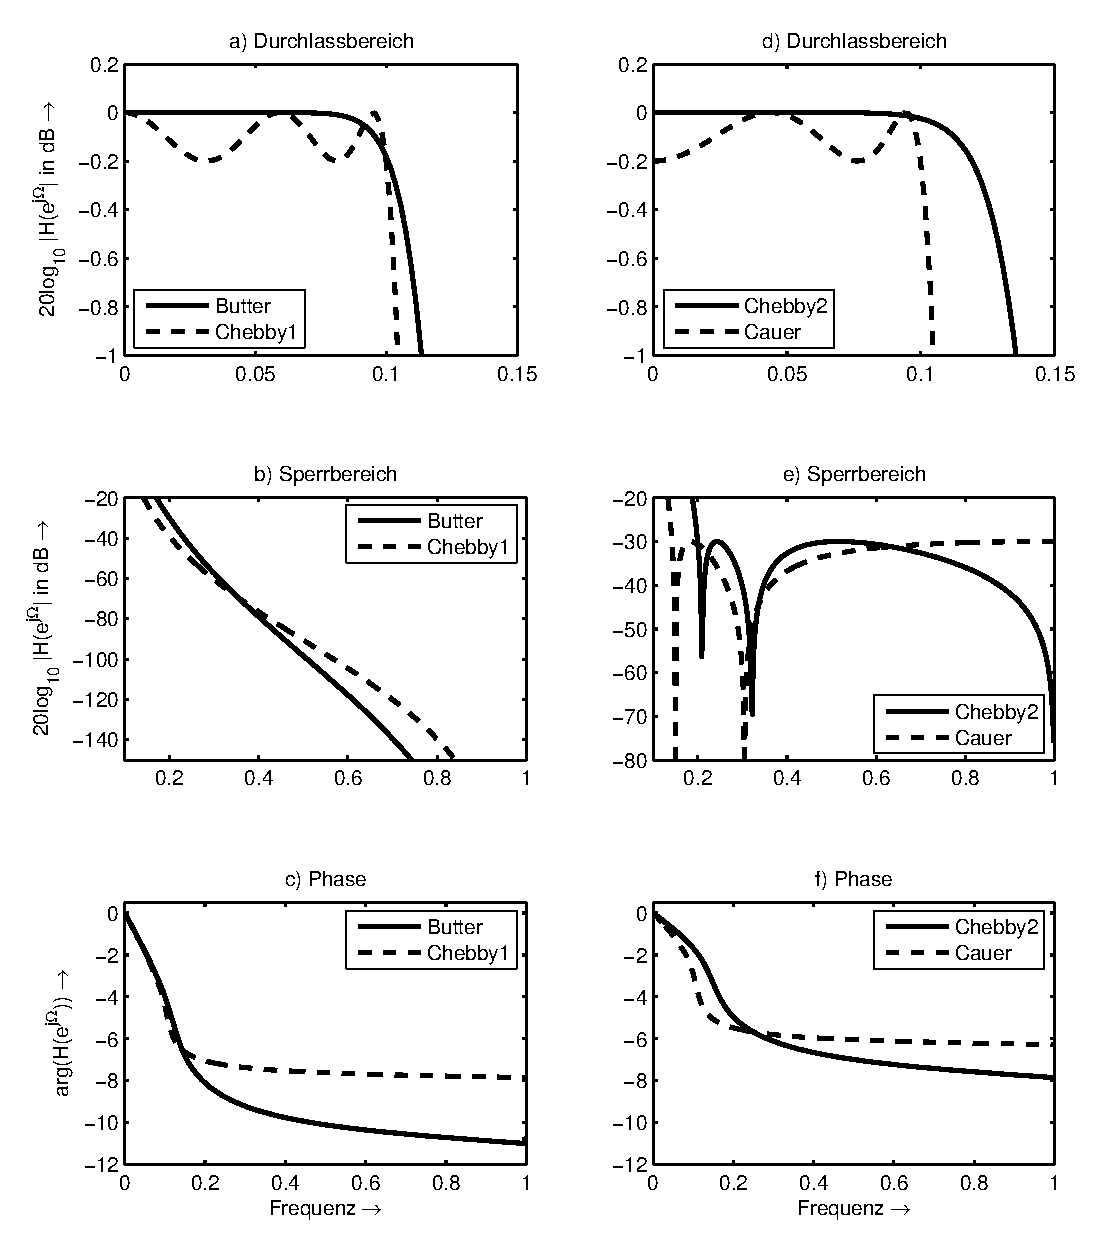
\includegraphics{psFilt/IIRDesign}
\caption{\label{pic:IIR:DesignBsp}Beispiel eines Tiefpass-Entwurfes für verschiedene Entwurfsverfahren.}.
\end{center}
\end{figure}

Das Butterworth-Filter hat im Durchlassbereich den erwarteten positiven flachen Verlauf, der im Sperrbereich
zu einer monoton fallenden Dämpfung führt. Dieses Verhalten im Sperrbereich wird auch vom
Tschebyscheff-I-Filter im Sperrbereich erreicht, wobei trotz der geringeren Ordnung ein
zunächst steilerer Übergang an der Grenzfrequenz erreicht wird. Beim Tschebyscheff-II-Filter
im Durchlassbereich wird deutlich, dass die Spezifikation übererfüllt wird. Die Grenzfrequenz
bei der der Übergang beginnt, ist verschoben, da beim Tschebyscheff-II-Design in erster
Linie der Sperrbereich erfüllt werden soll.

Ein bisher nicht beachteter Aspekt ist in den Bildern c und f gezeigt. Hier wird deutlich,
dass die Phase im Übergangsbereich durch das Cauer-Filter am stärksten verzerrt wird, während das
Butterworth-Filter am ehesten der meistens gewünschten linearen Phase entspricht.

\tbd {Impuls bzw. Step-Verhalten zur Glättung}

\subsubsection{Entwurf von Hochpass, Bandpass und Bandsperr-Filter}
Bisher wurden nur Tiefpass-Entwürfe betrachtet. Alle anderen Filter lassen sich ebenfalls
errechnen, wobei die dazu verwendeten Frequenz-Transformationen\footnote{Nicht zu verwechseln mit
der Fourier-Transformation} erst bei der Betrachtung der analogen Prototyp-Filter genauer
erläutert werden soll.

Für den Entwurf mit Matlab ergibt sich für alle Verfahren das gleiche Schema. Ein Hochpass-Filter
wird durch einen speziellen Schalter (Flag = ''high'') angezeigt. Der Bandpass-Entwurf ergibt sich
automatisch, wenn mehr als eine Grenzfrequenz angegeben wird, während die Bandsperre mit zwei
Grenzfrequenzen und einem Flag = ''stop'' angezeigt wird. Zur Berechnung der Ordnung
reicht es die Grenzfrequenzen zu vertauschen, um einen Hochpass anzuzeigen.

Matlab-Beispiel:

\begin{verbatim}
% Highpass-Design
Pass_freq = 0.2; % Matlab uses normalized frequencies from 0..2
Pass_dB = 0.2;
Stop_freq = 0.1;
Stop_dB = 30;

[N,f_g] = buttord(Pass_freq,Stop_freq,Pass_dB,Stop_dB);
% Result is 7th Order and f_g = 0.1247
[b,a] = butter(N,f_g,'high');

%Bandpass Design
Pass_freqLow = 0.2; % Matlab uses normalized frequencies from 0..2
Pass_freqHigh = 0.3; % Matlab uses normalized frequencies from 0..2
Pass_dB = 0.2;
Stop_freqLow = 0.1;
Stop_freqHigh = 0.4;
Stop_dB = 30;
[N,f_g] = buttord([Pass_freqLow Pass_freqHigh],[Stop_freqLow Stop_freqHigh],Pass_dB,Stop_dB);
[b,a] = butter(N,f_g);

% Bandstop Design
Pass_freqLow = 0.1; % Matlab uses normalized frequencies from 0..2
Pass_freqHigh = 0.4; % Matlab uses normalized frequencies from 0..2
Pass_dB = 0.2;
Stop_freqLow = 0.2;
Stop_freqHigh = 0.3;
Stop_dB = 30;
[N,f_g] = buttord([Pass_freqLow Pass_freqHigh],[Stop_freqLow Stop_freqHigh],Pass_dB,Stop_dB);
[b,a] = butter(N,f_g,'stop');

\end{verbatim}

%\section{Quantisierungseinflüsse beim Entwurf und bei der Filterung}
%\subsection{Pol-Nullstellenlagen}
%\subsection{SNR-Verschlechterung durch Quantisierungsrauschen}


\section{Übungen}
\subsection{Wiederholung des Stoffes und einfache Rechenaufgaben}
\begin{enumerate}
    \item Nennen Sie jeweils eine mögliche Anwendung (am besten aus dem Bereich
    der Audiotechnik, Hörtechnik, Audiologie) für die verschiedenen Grundcharakteristika
    und überlegen sich, wie die Entwurfsparamter aussehen könnten (Grenzfrequenz, Ordnung)
    \item Geben Sie zu folgendem Blockschaltbild die Differenzengleichung an.
        \begin{figure}[H]
        \begin{center}
        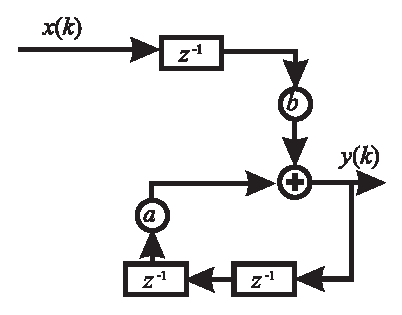
\includegraphics{psUeb/IIr_2terOrdnung}
        \caption{\label{pic:IIR_System} Blockschaltbild eines Systems}
        \end{center}
        \end{figure}
    \item Welche Vor- und Nachteile ergeben sich durch das Overlap-Add Verfahren zur schnellen
    Faltung?
    \item Zeichnen Sie zu den folgenden Systemen eine Realisierung als Blockschaltbild
    \begin{enumerate}
        \item $y(k) = x(k) - \alpha y(k-1)$
        \item $y(k) =  0.3 x(k) + 07 x(k-1) + 1.9812 y(k-1)   - 1.0201 y(k-2)$
    \end{enumerate}
\end{enumerate}

\subsection{Aufgaben (Auf Klausurniveau)}
\begin{enumerate}
    \item Berechnen Sie die Übertragungsfunktion der Impulsantwort
    $h(k) = [-1 \;\; 1]$! Skizzieren Sie den Betrags- und Phasengang!
    Um was für einen Filtertyp handelt es
    sich (Realisierungsform und Filtercharakteristik)?
   \item Sie sehen die folgende Impulsantwort. Um was für ein Filter
    handelt es sich (Realisierung und Filtercharakteristik)?
    Berechnen Sie die Übertragungsfunktion und skizzieren Sie den
    Betrags- und Phasenverlauf! Was ist besonders an diesem Filter
    und könnte es realisiert werden?
    \begin{figure}[H]
    \begin{center}
    \includegraphics{psUeb/KlausurWS2003_2IR}
    \end{center}
    \end{figure}
    \item Gegeben ist das folgende System
    \[
        y(k) = 2x(k) + 2x(k-1) - 2x(k-3) - 2x(k-4)
    \]
    Berechnen Sie die Übertragungsfunktion nach Betrag und Phase! Skizzieren Sie
    den Betrags- und Phasenverlauf zwischen 0 und $\pi$! Um was für einen Typ Filter handelt es sich?
    Zeichnen Sie eine möglichst effiziente Realisierung als Blockschaltbild!

    \item Skizzieren Sie den Betragsverlauf zu dem hier vorliegenden Pol-Nullstellenplan! Welche
    besonderen Eigenschaften hat dieses System? Geben Sie die Übertragungsfunktion $H(z)$ als Funktion von
    Biquads an. Nehmen Sie an, die Radien für die Pole und Nullstellen betragen $0.9$ bzw $1.1$ und $b_0 = 1$.
    \begin{figure}[H]
    \begin{center}
    \includegraphics[width = 8cm]{psUeb/PZ_18_25_28}
    \end{center}
    \end{figure}
    \item Wie lautet die Differenzengleichung und die
    Übertragungsfunktion des folgenden Systems
    nach Betrag und Phase? Zeichnen Sie den Betrags- und Phasenverlauf!
    Um was für eine Art Filter handelt es sich?
    (Typ und Realisierungsform)
    \begin{figure}[H]
    \begin{center}
    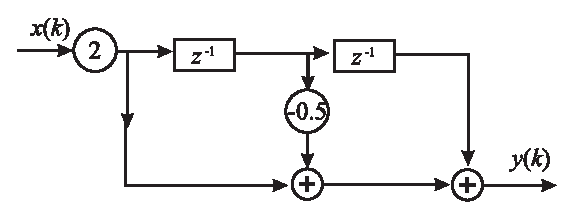
\includegraphics[width = 10cm]{psUeb/FIR_zweiterOrdnung}
    \end{center}
    \end{figure}

\end{enumerate}
\ifthenelse {\boolean{bBook}}
{
\subsection{Matlab-Aufgaben}
\begin{enumerate}
    \item Realisieren Sie eine Funktion, die die Koeffizienten eines mit der Fenstermethode
    entworfenen Tiefpasses zurückgibt. Als Übergabeparameter sollten die Grenzfrequenz, die Ordnung und das
    zu verwendende Fenster zur Verfügung stehen. Als Standard-Fenster soll das Rechteck-Fenster
    verwendet werden.
    \item Schreiben Sie eine Funktion, die aus einem beliebigen FIR-Filter eine minimalphasige
    Realisierung macht, wobei die Betragsübertragungsfunktion exakt erhalten bleiben soll.
    Die Übergabeparameter sind nur die bisher verwendeten FIR-Koeffizienten.
\end{enumerate}
}{}
\subsection{Transfer-Leistung}
\begin{enumerate}
    \item Überlegen Sie eine weitere kanonische Struktur für SOS-Filter.
    \item Nehmen wir an beim OLA-Verfahren wechselt die Übertragungsfunktion
    während der Datenvektor noch nicht vollständig bearbeitet wurde (Zeitvariantes Verhalten).
    Was glauben Sie ist die Folge? Können Sie sich vorstellen, wie man die auftretenden
    Probleme lösen kann?
\end{enumerate}

\ifthenelse {\boolean{bZusammenfassung}}
{%
\section{Zusammenfassung}
Die wichtigen Erkenntnisse aus diesem Kapitel sind:
\begin{itemize}
    \item LTI-Systeme ergeben für alle nicht-trivialen Fälle eine Filterung des Signals. Die
    Filterwirkung kann, muss aber nicht Ziel der Signalverarbeitung sein. Beispiel: gleitender Mittelwert.
    Ziel ist Mittelung, Nebenwirkung ist Filterung.
    \item Das ideale Tiefpass-Filter ist nicht realisierbar. Die Impulsantwort ist durch die si-Funktion gegeben
    und deshalb nicht-kausal und unendlich ausgedehnt.
    \item Man unterscheidet FIR (Finite Impulse Response) und IIR (Infinite Impulse Response)-Filter.
    \item FIR-Filter können durch Abschneiden und Verschieben der idealen Imulsantwort approximiert werden. Es
    ergeben sich durch diesen Entwurf immer linearphasige Filter.
    \item Es gibt 4 unterschiedliche linearphasige Filter, die sich durch die Symmetrie der
    Filterkoeffizienten unterscheiden.
    \item Nur mit dem Typ I Filter lassen sich alle Filtercharakteristike realisieren.
    \item Minimalphasige Filter können aus dem linearphasigen Entwurf berechnet werden.
    \item IIR-Filter werden zur Realisierung in Systeme 2ter Ordnung (Second Order Sections (SOS))
    zerlegt.
    \item Die konkrete Realisierung eines Filters kann als Blockschaltbild dargestellt werden
    \item Für IIR Filter gibt es unterschiedliche Strukturen mit gleicher Filterwirkung.
    Strukturen mit einer minimalen Anzahl an Speicherplätzen werden kanonisch genannt.
    \item Die geschickteste Realisierung zur FIR-Filterung langer Signale und hoher Filterordnungen
    erfolgt mit der Overlap Add Methode.
    \item Matlab bietet viele Hilfsmittel für den Entwurf von IIR-Filtern.
\end{itemize}
}{} 